%%% PREAMBLE - Do not touch %%%%%%%%%%%%%%%%%%%%%%%%%%%%%%%%%%%%%%%%%%%%%%%%%%%%%%
\documentclass[10pt,twocolumn,letterpaper]{article}
\usepackage[utf8]{inputenc}
\usepackage[brazil]{babel}
\usepackage{bm}
\usepackage{model}
\usepackage{times}
\usepackage{epsfig}
\usepackage{graphicx}
\usepackage{amsmath}
\usepackage{amssymb}
\usepackage{color}
\usepackage[pagebackref=true,breaklinks=true,letterpaper=true,colorlinks,bookmarks=false]{hyperref}
\input{pics/abaco}

\cvprfinalcopy % *** Uncomment this line for the final submission
\def\httilde{\mbox{\tt\raisebox{-.5ex}{\symbol{126}}}}
\ifcvprfinal\pagestyle{empty}\fi


%%% Report beginning %%%%%%%%%%%%%%%%%%%%%%%%%%%%%%%%%%%%%%%%%%%%%%%%%%%%%%%%%%%%%%
\begin{document}

%%% Title and authors %%%%%%%%%%%%%%%%%%%%%%%%%%%%%%%%%%%%%%%%%%%%%%%%%%%%%%%%%%%%
\title {Agrupando títulos de notícias de jornal em grupos similares com o k-means}
\author{Gustavo Ciotto Pinton, RA117136\thanks{Is with the Institute of Computing, University of Campinas (Unicamp). \textbf{Contact}: \tt\small{gustavociotto@gmail.com}}\\
Lucas Rath Maia, RA117751\thanks{Is with the Institute of Computing, University of Campinas (Unicamp). \textbf{Contact}: \tt\small{lucasrm25@gmail.com}}}

%%% Abstract %%%%%%%%%%%%%%%%%%%%%%%%%%%%%%%%%%%%%%%%%%%%%%%%%%%%%%%%%%%%%%%%%%%%%
\maketitle
\begin{abstract}
Neste documento, são propostos dois métodos capazes de agrupar títulos de jornais em categorias de acordo com o seu tema.  Ambos os métodos utilizam a técnica de clusterização denominada de k-means, porém a maneira com que os atributos foram gerados variou. O primeiro método utilizou a técnica de bag-of-words aliada ao cálculo da métrica TFIDF sobre word n-grams, com \(n\) indo de 1 a 5, enquanto que o segundo baseou-se no uso de matrizes previamente calculadas, chamadas de word embeddings.  No total, foram disponibilizados um milhão de títulos publicados entre 2003 e 2017 do jornal australiano ABC (Australian Broadcasting Corporation).
\end{abstract}

%%% Introduction %%%%%%%%%%%%%%%%%%%%%%%%%%%%%%%%%%%%%%%%%%%%%%%%%%%%%%%%%%%%%%%%%
\section{Introdução}
\label{intro}

Técnicas de agrupamento de elementos em grupos com características semelhantes possuem cada vez mais interesse nos dias de hoje com a ampla utilização das redes sociais. Elas permitem, por exemplo, que propagandas e campanhas sejam direcionadas a determinados grupos de maneira que o efeito sobre os elementos que o compõem seja potencializado. Outro exemplo do grande poder deste tipo de técnica foi o recente caso da empresa \textit{Cambridge Analytica} que utilizou um grande volume de perfis da rede social Facebook para categorizar indivíduos em grupos com orientações políticas semelhantes com o objetivo de influenciar eleições de diversos países, incluindo a dos Estados Unidos \cite{CA}.

Tendo em vista tal capacidade, propomos neste documento a clusterização de títulos publicados entre 2003 e 2017 do jornal australiano ABC (\textit{Australian Broadcasting
Corporation}), a partir da técnica de aprendizado não supervisionado denominada \textit{k-means}. Tal técnica consiste no cálculo de \(k\) centroídes, de maneira a otimizar as distâncias de cada amostra a seu determinado centroíde. Assim como qualquer método de aprendizado de máquina, a otimização implica a minimização de uma função de custo \(J\), conforme representado na equação \ref {eq:cost}, logo abaixo, em que  \(M\) é a quantidade de amostras disponíveis, \(\bm{c}^{(i)}\) é o índice do centróide ao qual a amostra \(\bm{x}_i\) pertence e \(\bm{\mu}_j\) é o centróide \(k\), com \(\bm{x}^i \text{ e } \bm{\mu}_j \in \mathbb{R}^n \). Por fim, a quantidade de centróides a ser utilizada é obtida a partir de um método tal como o \textit{elbow method}, de modo que o \(k\) escolhido fique entre uma região de distorção estabilizada e outra em que a mesma métrica cai rapidamente.

\begin{equation}
\label {eq:cost}
J(\bm{c}^{(1)}, ..., \bm{c}^{(m)}, \bm{\mu}_1, ..., \bm{\mu}_k) =  \frac{1}{M} \displaystyle\sum_{i=1}^{M} \left\Vert \bm{x}_i - \bm{\mu}_{\bm{c}^{(i)}} \right\Vert ^2
\end{equation}

Antes de utilizarmos o \textit{k-means}, é necessário obtermos atributos pertinentes e que descrevam corretamente cada um dos títulos das notícias, isto é, necessita-se traduzir uma frase em um vetor \(\bm{x}_i\) numérico aplicável ao \textit{k-means}.  Neste documento, serão apresentados dois mecanismos de obtenção destes atributos. O primeiro é baseado na técnica de \textit{bag-of-words} \cite{7555393} aliada ao cálculo da métrica \textit{TFIDF} sobre \textit{word n-grams} gerados a partir de cada título. Neste caso, separa-se os títulos em \textit{tokens} e, de acordo com \(n\), inclui-se na \textit{bag-of-words} toda combinação sequencial contendo \(n\) destes \textit{tokens}. Por exemplo, para a frase \textit{I love cat} e \(n = 2\), consideraríamos \textit{I love} e \textit{love cat}. Uma vez inseridas todas as combinações na \textit{bag-of-words}, a próxima etapa, para cada título, é calcular a frequência (ou \textit{term frequency}) que cada combinação aparece neste determinado título multiplicada pelo fator \textit{inverse document frequency}, que avalia a importância desta combinação entre todos os títulos. Em outras palavras, dá-se menos importância a \textit{n-grams} que aparecem em muitos títulos pelo simples fato de que eles não acrescentam informação nova e específica, não sendo, portanto, importantes para a diferenciação e agrupamento dos respectivos títulos. Palavras como \textit{the}, por exemplo, podem ter uma frequência alta em um título, porém também podem receber um fator \textit{IDF} extremamente baixo, tendo em vista que aparecem em muitas amostras distintas. A equação \ref {eq:tfidf} representa uma maneira para calcular a métrica \textit{TFIDF}, em que \(f_{t,d}\) é a frequência do termo (ou \textit{n-gram}) \(t\) no título \(d\), \(M\) é o número total de amostras e \(m_t\) é o número de amostras em que \(t\) aparece.

\begin{equation}
\label {eq:tfidf}
\text{TFIDF} (t) = \frac{f_{t,d}}{\displaystyle\sum_{t' \in d} f_{t',d}}\log\left(\frac{M}{m_t}\right)
\end{equation}

Como o leitor deve estar imaginando, a matriz de atributos gerada a partir do método descrito acima é extremamente esparsa, isto é, preenchida em sua quase totalidade por 0. Tendo em vista que o \textit{k-means} não é muito eficiente para este tipo de estrutura de dados, precisamos de algo que reduza a dimensionalidade dos vetores de atributos. Nesse contexto, utiliza-se ou o PCA ou o SVD para tal redução. Ambos utilizam o cálculo de autovetores e autovalores sobre a matriz de auto-covariância com o intuito de calcular as \(n\) direções de maior variância, porém o segundo, ao contrário do primeiro, não centraliza os dados antes de computar a decomposição dos valores singulares, sendo muito mais eficiente para matrizes esparsas. Neste relatório, será utilizada, portanto, a técnica de SVD.

A segunda técnica de processamento de atributos é denominada \textit{word embeddings}. Neste caso, uma matriz \(\bm{W}_{P \times D}\) relaciona uma determinada palavra \(i \in [1, P]\) a um vetor de dimensão \(D\) da ordem de centenas de elementos. Multiplica-se \(\bm{W}\) com a matriz \(\bm{F}_{M \times P}\) em que cada linha contém \(P\) elementos, em que cada um deles representa a quantidade de ocorrências da palavra \(i\) no respectivo título. Obtém-se, assim, a nova matriz \(\bm{V}_{M \times D}\) contendo os atributos a serem utilizados no \textit{k-means}. Neste documento, a matriz \(\bm{W}\) foi gerada a partir de um algoritmo chamado \textit{GloVe} \cite{pennington2014glove} e dados retirados da \textit{Wikipedia} no ano de 2014. Uma característica interessante da matriz gerada por esse algoritmo é que palavras com contextos correlacionados terão vetores apontando para direções semelhantes. Por exemplo, \textit{king} e \textit{queen} têm vetores parecidos. Além disso, verifica-se a relação vetorial \textit{king} - \textit{queen} = \textit{man} - \textit{woman}. Em suma, o próprio algoritmo se encarrega de adicionar o significado semântico de palavras correlacionadas, possibilitando uma clusterização eficiente.

É importante ressaltar que antes dos dois processamentos apresentados, transformam-se eventuais letras maiúsculas em minúsculas e retiram-se dos documentos todas \textit{stop words}, isto é, palavras que não acrescentam nenhuma informação adicional tal como artigos e preposições. Adicionalmente, optamos por reduzir do vocabulário palavras com frequência acima de uma porcentagem determinada a partir de testes. Isso foi realizado para evitar que os métodos gerassem clusters viciados em apenas palavras iguais e não significados.

Por fim, por limitações computacionais, resolvemos utilizar apenas uma fração dos dados, isto é, apenas o ano de 2017, para o agrupamento. Assume-se, portanto, que os temas não variam muito de um ano para o outro.
%%% Add section %%%%%%%%%%%%%%%%%%%%%%%%%%%%%%%%%%%%%%%%%%%%%%%%%%%%%%%%%%%%%%%%%%
\section{Atividades}

As próximas subseções visam explicar as escolhas dos diversos parâmetros adotados pelo autor.

\subsection {Cálculo dos atributos com bag-of-words}

Conforme discutido na seção \textbf {Introdução}, utilizamos apenas \textit{word n-grams} para o cálculo da métrica \textit{TFIDF}. Após testes, determinou-se que os melhores resultados foram para \(n\) no intervalo [1,5]. A figura \ref{img:hist} nos ajuda a entender um pouco o porquê deste resultado: a maioria dos títulos contém entre 4 e 7 palavras, sendo assim, \textit{n-grams} com \(n\) mais elevados nos ajudam a representar melhor o significado de cada sentença e impedem que os \textit{clusters} se viciem em apenas palavras semelhantes. Para esta configuração e ano de 2017, os 44182 vetores de atributos obtidos possuíram 5885 elementos. Também a partir de testes, escolhemos reduzir tal dimensionalidade para 50 utilizando a técnica de \textit{Single Value Decomposition} (SVD), conforme discutido na seção anterior. Para os dois passos, empregamos bibliotecas já implementadas no módulo \textit{python sklearn} \cite{scikit-learn}.

\begin{figure}
    \centering
    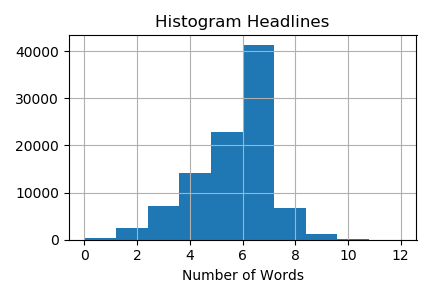
\includegraphics[width=\columnwidth]{figs/histograma_n_palavras}
    \caption{Histograma do número de palavras nos títulos das notícias para o ano de 2017. Pré-processamento (eliminação de \textit{stop words}, letras maiúsculas) já realizado.}
    \label{img:hist}
\end{figure}

\subsection {Cálculo dos atributos com word embeddings}

A partir do algoritmo GloVe \cite{pennington2014glove}, escolhemos o \textit{dataset} com 400 mil palavras no vocabulário e vetores de 300 elementos. Neste caso, evidentemente, utilizamos apenas \(n=1\) para o cálculo dos \textit{word n-grams} e obtivemos vetores de atributos com 300 elementos para uso direto no \textit{k-means}.

\section {Soluções propostas}

Essa seção é dedicada à discussão das soluções propostas.

\subsection{Bag-of-words e SVD}

A primeira etapa é determinar o número de \textit{clusters} a ser utilizados. Para tal, realizamos a processamento para \(k\) de 2 até 80 e, a partir do \textit{elbow method}, determinamos experimentalmente qual deles é a melhor opção. A figura \ref{img:kmeans_svd} possui os resultados das distorções, definidas como a soma das distâncias ao quadrado entre cada amostra e o seu centroíde dominante, para todo o intervalo sugerido. Verifica-se que, apesar da grande variação, o \textit{cotovelo} é encontrado para \(k = 40\), ponto em que a soma das distâncias estabilizam-se em torno de aproximadamente 1375 (salvo apenas algumas exceções como \(k = 50\) e \(k\) inferiores a $\sim$70). Ressalta-se que para todos os cálculos, o número de iterações máximos do \textit{k-means} foi 1000.

\begin{figure}
    \centering
    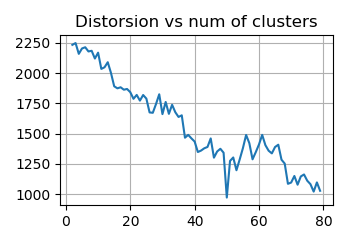
\includegraphics[width=\columnwidth]{figs/elbow_kmeans_tfidf_1-5_svd}
    \caption{Distorção para cada valor de \(k\) variando de 2 até 80 para atécnicas de \textit{bag-of-words} e SVD.}
    \label{img:kmeans_svd}
\end{figure}

Tendo escolhido o valor de \(k\), podemos utilizar uma ferramenta de visualização para verificar se os \textit{clusters} foram bem definidos. Uma alternativa é o \textbf{t-SNE}, que consiste em uma técnica de redução de dimensionalidade adequada para a visualização de \textit{datasets} com muitas dimensões. A figura \ref{img:tsne_svd} representa o resultado da clusterização para \(k = 40\) para apenas 2000 amostras (tal limitação foi devida aos recursos computacionais disponíveis). Observa-se a presença de grupos muito bem separados e definidos nas partes mais externas do gráfico e um grupo predominante no centro. Este último possui títulos, ao contrário dos demais, com temas não muito definidos, sendo considerados pelo autor deste documento como \textbf{Geral}. Abaixo, são apresentadas as tuplas \((W, Q)\) para alguns dos \textit{clusters} obtidos neste método, em que \(W\) é um \textit{word n-gram}
e \(Q\) é a quantidade de vezes que \(W\) aparece. Tal listagem ocorre em ordem decrescente em relação a \(Q\) e considera apenas os cinco maiores \(Q\). Além disso, são adicionadas três títulos escolhidos randomicamente no respectivo \textit{cluster} e uma breve explicação sobre o seu tema.

\begin{figure}
    \centering
    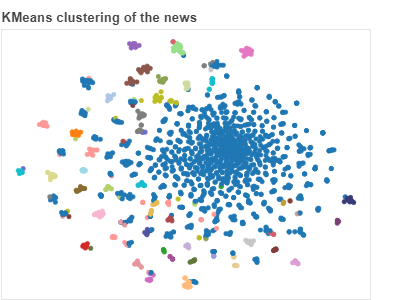
\includegraphics[width=\columnwidth]{figs/bokeh_plot_tfidf_1-5_svd_no_legend}
    \caption{Representação obtida a partir da técnica de t-SNE para 40 \textit{clusters}.}
    \label{img:tsne_svd}
\end{figure}

\begin{itemize}
  \item \textbf {Cluster 1}: 31831 títulos no total. (house, 292), (health, 280), (school, 270), (woman, 268), (labor, 265). Frases: (i) \textit{political donations in queensland to be revealed within 7 days}, (ii) \textit{should tourists boycott myanmar again}, (iii) \textit{nsw hot weather boils with penrith record}. As frases neste \textit{cluster} não possuem nenhum tema específico em comum, sendo, deste modo, classificados no tema \textbf{Geral}.

  \item \textbf {Cluster 3}: 199 títulos no total. (scorecentre, 159), (nrl, 127), (afl, 75), (raiders, 29), (broncos, 29), (bulldogs, 26). Frases: (i) \textit{nrl scorecentre warriors broncos sharks bulldogs}, (ii) \textit{nrl top five: april 3}, (iii) \textit{nrl scorecentre}. O assunto deste \textit{cluster} é facilmente identificado como \textbf{Liga de Rugby Australiana}, contendo títulos com a abreviação \textit{nrl} e nomes de diversos times.

  \item \textbf {Cluster 5}: 638 títulos no total.  (murder, 360), (charged, 353), (alleged, 47), (woman, 36), (trial, 33), (stabbing, 31). Frases: (i) \textit{      rockhampton man ian coombe charged with fraud}, (ii) \textit{former teacher charged over alleged historical sex assaults}, (iii) \textit{borce ristevski faces court charged with murdering wife karen}. Este \textit{cluster} agrupa títulos relacionados a \textbf{Crimes e assassinatos}.

  \item \textbf {Cluster 20}: 127 títulos no total.  (violence, 127), (domestic, 110), (victims, 16), (demand, 6), (help, 6). Frases: (i) \textit{russian women hide domestic violence scars with tattoos}, (ii) \textit{candlelight vigil in hobart for domestic violence victims}, (iii) \textit{catalonia how did it come to violence in the streets}. Este \textit{cluster} é dominado pelas palavras \textit{violence} e \textit{domestic} que aparecem muito mais que as demais. Portanto, o tema do grupo é  \textbf{Violência doméstica}.

  \item \textbf {Cluster 21}: 323 títulos no total. (marriage, 325), (vote, 40), (survey, 37), (bill, 25), (postal, 22), (gay, 15). Frases: (i) \textit{margaret court marriage bible isnt meant to be read so literally}, (ii) \textit{the same sex marriage debate}, (iii) \textit{same sex marriage bill debate moves to amendments}. O tema predominante neste \textit{cluster} é \textbf{Casamento de pessoas do mesmo sexo}, apesar de que apenas a palavra \textit{marriage} aparece muito mais que as demais. Nota-se também que \textit{marriage} ocorre mais de uma vez em um mesmo título, tendo em vista que suas aparições superam o próprio número de títulos no \textit{cluster}.

  \item \textbf {Cluster 30}: 406 títulos no total. (crash, 321), (killed, 71), (fatal, 68), (plane, 63), (dead, 56), (car, 53), (driver, 49). Frases: (i) \textit{uber suspends self driving car program after arizona crash}, (i) \textit{plane crash on swan river during australia day}, (iii) \textit{police searching for driver of truck that hit sydney home}. A principal temática deste grupo, conforme palavras e frases, é \textbf{Acidente em meios de transporte}.

  \item \textbf {Cluster 38}: 179 títulos no total. (media, 163), (social, 115), (video, 10), (campaign, 8), (facebook, 8).  Frases: (i) \textit{film media union to look at safety after bliss n eso shooting}, (ii) \textit{pepsi pulls kendall jenner ad amid social media outcry}, (iii) \textit{formula one relaxes social media rules for teams}. Neste caso, notícias com o tema \textbf {Rede social} são agrupadas no \textit{cluster}.

\end{itemize}

\subsection{Word embeddings}

Assim como na solução anterior, é necessário selecionar a quantidade \(k\) de \textit{clusters} a ser utilizados com auxílio do \textit{elbow method}. Neste caso, temos vetores de atributos com 300 elementos gerados pela multiplicação da matriz de entrada por uma outra pré-processada a partir de dados do algoritmo GloVe, conforme discutido na seção \textbf{Introdução}. A figura \ref{img:kmeans_embedded} representa o resultado das distorções calculadas para \(k\) no intervalo de 2 a 80. Neste caso, escolhemos, \(k = 20\) para o número de centróides. Destaca-se que a distorção deste método é muito superior àquela calculada na solução anterior, sendo aproximadamente \(\frac{5.500.000}{1375} = 4000\) maior. A figura \ref{img:tsne_embedded}, por sua vez, possui o resultado da representação visual gerada pelo algortimo \textbf{t-SNE}. Observa-se que nenhum \textit{cluster} é visualmente bem definido, isto é, os dados estão dispostos em uma grande nuvem sem nenhuma separação aparente. Tal fato explica a grande diferença de distorção encontrado neste caso em relação ao anterior.

\begin{figure}
    \centering
    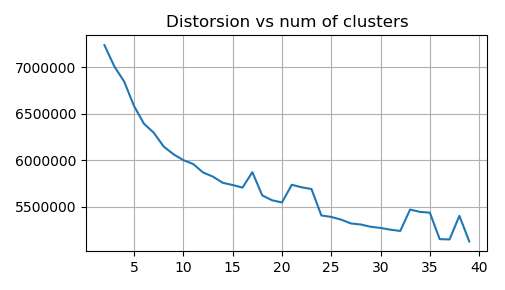
\includegraphics[width=\columnwidth]{figs/elbow_kmeans_embedded_1-5}
    \caption{Distorção para cada valor de \(k\) variando de 2 até 80 para a técnica de \textit{word embedding}.}
    \label{img:kmeans_embedded}
\end{figure}

\begin{figure}
    \centering
    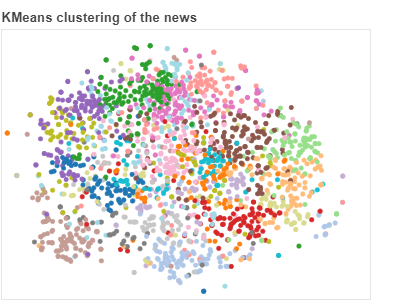
\includegraphics[width=\columnwidth]{figs/bokeh_plot_embedded_1-5_svd_no_legend}
    \caption{Representação obtida a partir da técnica de t-SNE para 20 \textit{clusters} com \textit{features} calculados a partir dos \textit{word embeddings}.}
    \label{img:tsne_embedded}
\end{figure}

Assim como na subseção anterior, destacam-se alguns \textit{clusters} obtidos a partir do método de \textit{word embeddings}:

\begin{itemize}
  \item \textbf {Cluster 3}: 1871 títulos no total. (cancer, 117), (hospital, 82), (health, 70), (disease, 65), (child, 65). Frases: (i) \textit{pressure on tweed hospital sends patients to qld}, (ii) \textit{chef prepares recipes for cancer patients}, (iii) \textit{a message about mens mental health}. O tema predominante neste \textit{cluster} são \textbf{Problemas relacionados à saúde}.

  \item \textbf {Cluster 8}: 1767 títulos no total. (turnbull, 82), (minister, 81), (malcolm, 66), (house, 64), (interview, 63). Frases: (i) \textit{premier opposition leader make final pitch wa election}, (ii) \textit{obama breaks healthcare silence to slam republican proposal}, (iii) \textit{why tasmanias western arthur range is such a tough walk}. As notícias neste \textit{cluster} tratam de \textbf{Política}.

  \item \textbf {Cluster 15}: 2134 títulos no total. (market, 177), (wall, 153), (prices, 145), (street, 121), (dollar, 110). Frases: (i) \textit{wage growth remains at record lows}, (ii) \textit{veroguard manufacturing centre create 600 jobs northern adelaide}, (iii) \textit{fossil beer the latest innovation to hit booming craft brewing}. Este \textit{cluster} trata claramente de notícias ligadas ao \textbf{Mercado e setor econômico}.

  \item \textbf {Cluster 19}: 2075 títulos no total. (murder, 314), (charged, 207), (guilty, 205), (alleged, 158), (accused, 129). Frases: (i) \textit{terrorist neil prakash denies charges reports}, (ii) \textit{animal cruelty charges see woman jailed 31 dogs 43 cats}, (iii) \textit{police officer charged with filming sex act with colleague}. Com base nas palavras mais frequentes neste \textit{cluster}, conclui-se que o seu tema é \textbf{Crimes e assassinatos}.

\end{itemize}

%%% Add section %%%%%%%%%%%%%%%%%%%%%%%%%%%%%%%%%%%%%%%%%%%%%%%%%%%%%%%%%%%%%%%%%%
\section{Conclusões}

Dois métodos de extração de atributos foram aplicados aos dados: \textit{bag-of-words} com \textit{word n-grams} e \textit{word embeddings}. Para o primeiro, encontrou-se a partir do \textit{elbow method} que o melhor número de \textit{clusters} a ser utilizado seria \(k = 40\). Com este \(k\), obtivemos um distorção, isto é, a soma das distâncias ao quadrado entre cada amostra e o seu centroíde dominante, de aproximadamente 1375. Para o segundo método, adotamos \(k = 20\) e chegamos a uma distorção 4000 vezes maior. Utilizando a ferramenta de visualização \textit{t-SNE}, visualizamos \textit{clusters} bem definidos para o primeiro método, enquanto que para o segundo, apenas uma nuvem de pontos sem separação aparente dos pontos, justificando, deste modo, a diferença observado na distorção.  Em geral, foi possível a atribuição de temas aos \textit{clusters} gerados em ambos os métodos.

%%% References %%%%%%%%%%%%%%%%%%%%%%%%%%%%%%%%%%%%%%%%%%%%%%%%%%%%%%%%%%%%%%%%%%%
{\small
\bibliographystyle{unsrt}
\bibliography{refs}
}

\end{document}
